\chapter{Planificación y presupuesto}

\section{Planificación}

\subsection{Fases}
Tomando en consideración que la parte del proyecto referente al análisis del sonido tiene un fuerte componente teórico, se ha dedicado una sección inicial a recabar todo tipo de información relacionada con la materia para obtener una visión global y definir así un enfoque claro antes de empezar a analizar tanto las especificaciones como los requisitos. El resto de las fases son en su mayoría, comunes a cualquier proceso de elaboración de un proyecto de software.

\begin{itemize}
  \item \textbf{Fase 1:} Lecturas relacionadas con la materia del proyecto.
  \item \textbf{Fase 2:} Especificaciones y planificación.
  \item \textbf{Fase 3:} Análisis y diseño.
  \item \textbf{Fase 4:} Implementación.
  \item \textbf{Fase 5:} Pruebas.
  \item \textbf{Fase 6:} Documentación.
\end{itemize}

\newpage
\subsection{Definición y estimación de tiempo para las tareas de cada fase}

Las fases detalladas anteriormente tienen varias tareas como sub-elementos, en la siguiente lista se detalla dichos sub-elementos y la estimación aproximada para llevarla a cabo.

\begin{itemize}
   \item \textbf{Lecturas relacionadas con la materia del proyecto:}
   \begin{itemize}
    \item Como se comportan las señales.
    \item Muestreo de señales.
    \item Digitalización de señales.
    \item Identificación de patrones en señales.
    \item \underline{\textit{Duración aproximada}}: 10 días.
    \end{itemize}
\end{itemize}

\begin{itemize}
   \item \textbf{Especificaciones y planificación:}
   \begin{itemize}
    \item Objetivos.
    \item Fases.
    \item Tareas y temporización.
    \item Presupuesto.
    \item \underline{\textit{Duración aproximada:}} 4 días.
   \end{itemize}
\end{itemize}

\begin{itemize}
   \item \textbf{Análisis y diseño:}
   \begin{itemize}
    \item Análisis de requisitos.
    \item Diagramas de la aplicación.
    \item \underline{\textit{Duración aproximada:}} 20 días.
   \end{itemize}
\end{itemize}

\begin{itemize}
 \item \textbf{Implementación:}
 \begin{itemize}
  \item Selección de tecnologías.
  \item Configuración Raspberry Pi
  \item Detección de sonido
  \item Identificación de vehículos
  \item Configuración de la plataforma IOT
  \item Configuración de base de datos de almacenamiento masivo.
  \item Configuración de visualizador de los datos recolectados.
  \item Desarrollo de sistema que comunique cuando un vehículo es detectado a la plataforma web.
  \item Desarrollo de la plataforma web
  \item \underline{\textit{Duración aproximada:}} 60 días.
 \end{itemize}
\end{itemize}

Cabe destacar que al ser un proyecto en el que existen fuertes dependencias entre los objetivos, la fase de pruebas ha sido completada al mismo tiempo que la de desarrollo pues se necesitan resultados concluyentes en algunos aspectos para poder avanzar en objetivos posteriores.

\begin{itemize}
 \item \textbf{Pruebas:}
 \begin{itemize}
  \item Pruebas de detección de vehículos.
  \item Pruebas de escritura en base de datos.
  \item Pruebas de lectura de la base de datos.
  \item Pruebas de comunicación entre dispositivos y plataforma web.
  \item \underline{\textit{Duración aproximada:}} 60 días.
 \end{itemize}
\end{itemize}

La documentación al igual que las pruebas, ha ido desarrollándose al mismo tiempo que la implementación, como se puede observar en la \textit{figura 3.1}.

\begin{itemize}
 \item \textbf{Documentación:}
 \begin{itemize}
  \item Documentación del código.
  \item Documentación del proyecto.
  \item \underline{\textit{Duración aproximada:}} 60 días.
 \end{itemize}
\end{itemize}

\subsection{Diagramas de temporización}

La información acerca de la temporización queda expuesta en las siguientes figuras mediante un diagrama de fases y tareas \textit{(figura 3.1)}, un diagrama de pert \textit{(figura 3.2)} y otro de gantt \textit{(figura 3.3)} y \textit{(figura 3.4)}.

\begin{figure}[!ht]
  \begin{center}
    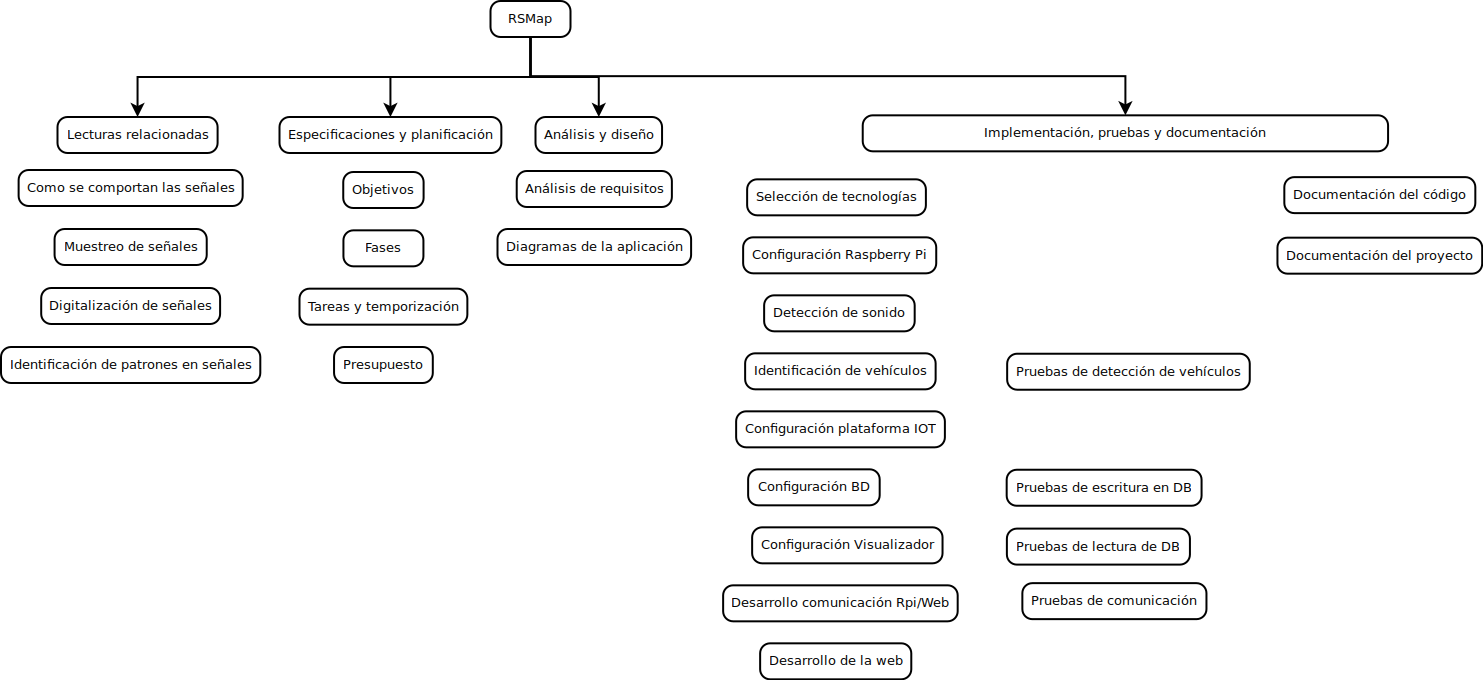
\includegraphics[scale=0.30]{../images/diag_plan/fases_tareas.png}
    \caption{Diagrama fases y tareas}
    \label{fig:fases_tareas}
  \end{center}
\end{figure}

\newpage
\begin{figure}[!ht]
  \begin{center}
    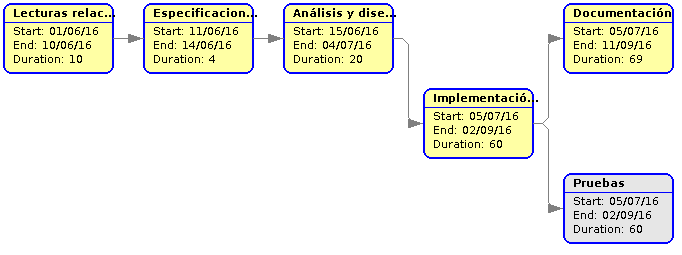
\includegraphics[width=1\textwidth]{../images/diag_plan/pert.png}
    \caption{Diagrama de pert}
    \label{fig:pert}
  \end{center}
\end{figure}

\begin{figure}[!ht]
  \begin{center}
    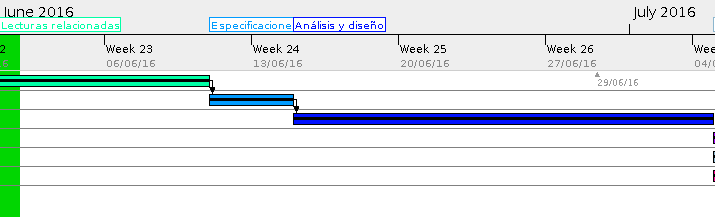
\includegraphics[width=1\textwidth]{../images/diag_plan/gantt1.png}
    \caption{Diagrama de Gantt 1}
    \label{fig:diag_gant1}
  \end{center}
\end{figure}

\begin{figure}[!ht]
  \begin{center}
    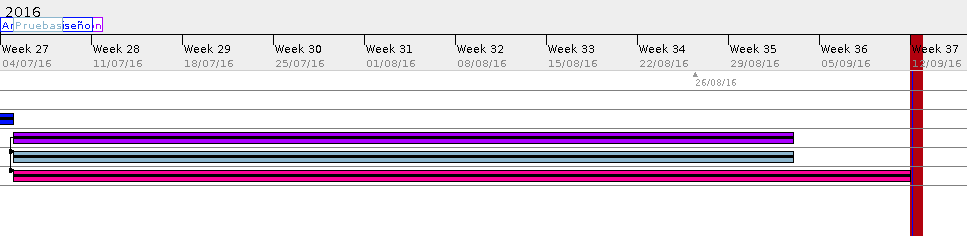
\includegraphics[width=1\textwidth]{../images/diag_plan/gantt2.png}
    \caption{Diagrama de Gantt 2}
    \label{fig:diag_gant2}
  \end{center}
\end{figure}

\newpage
\newpage

\section{Presupuesto}

En el presupuesto podemos distinguir entre el software y el hardware. Por una parte el aspecto software queda totalmente cubierto de manera gratuita ya que todas las tecnologías usadas son de código abierto por tanto esto nos ahorra muchos {\textit{- por no decir todos -} los costes de este tipo.

Por otra parte tenemos el componente hardware, que se detalla a continuación:

\newpage

\begin{itemize}
 \item \textbf{Raspberry Pi}
 \begin{itemize}
  \item Descripción: Dispositivo usado para la detección de datos.
  \item Especificaciones:  (\url{https://www.raspberrypi.org/products/raspberry-pi-2-model-b/})
  \item Precio: 31.98 Euros
 \end{itemize}
\end{itemize}
\begin{figure}[!h]
  \begin{center}
    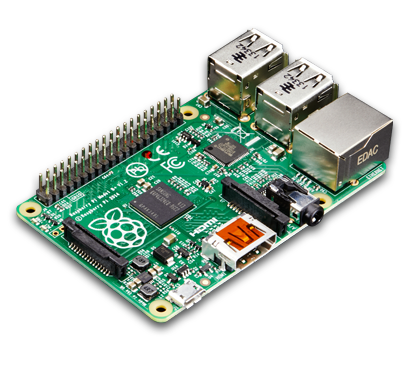
\includegraphics[scale=0.30]{../images/hardware/pi.png}
    \caption{Raspberry Pi 2B}
    \label{fig:rpi}
  \end{center}
\end{figure}

\begin{itemize}
 \item \textbf{Tarjeta de audio USB}
 \begin{itemize}
  \item Descripción: Interfaz por el cual capturamos el sonido.
  \item Especificaciónes: \url{http://www.logilink.org/showproduct/UA0078.htm}
  \item Precio: 9.37 Euros
 \end{itemize}
\end{itemize}
\begin{figure}[!h]
  \begin{center}
    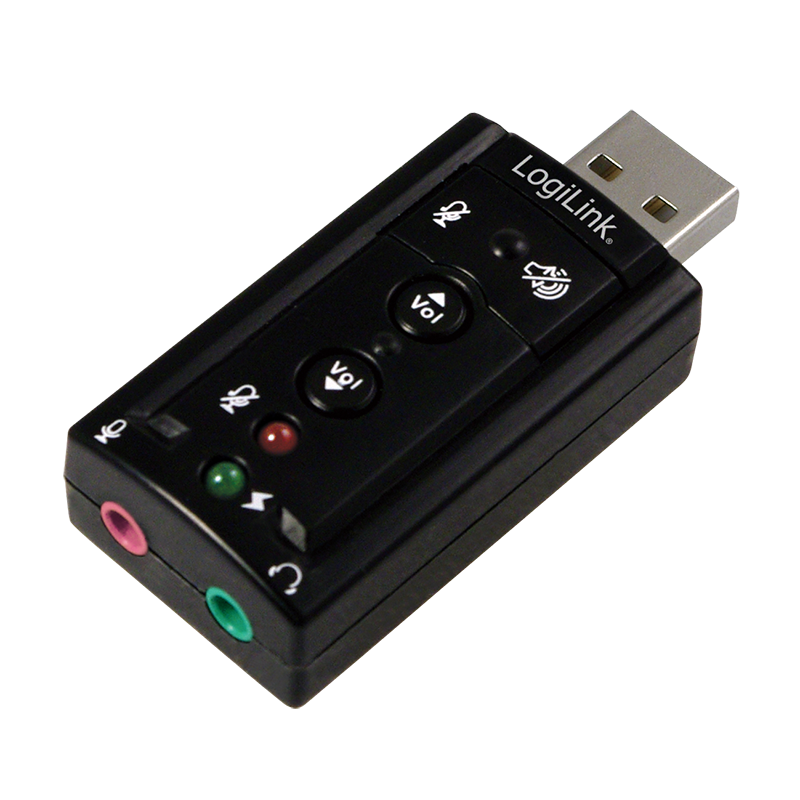
\includegraphics[scale=0.10]{../images/hardware/audiocard.png}
    \caption{Tarjeta de sonido}
    \label{fig:usbsonido}
  \end{center}
\end{figure}

\begin{itemize}
 \item \textbf{Micrófono}
 \begin{itemize}
  \item Descripción: Entrada a la interfaz de audio.
  \item Especificaciónes: \url{https://www.amazon.co.uk/Flexible-3-5mm-Microphone-Notebook-Laptop/dp/B00CRASVFC}
  \item Precio: ~5 Euros
 \end{itemize}
\end{itemize}
\begin{figure}[!ht]
  \begin{center}
    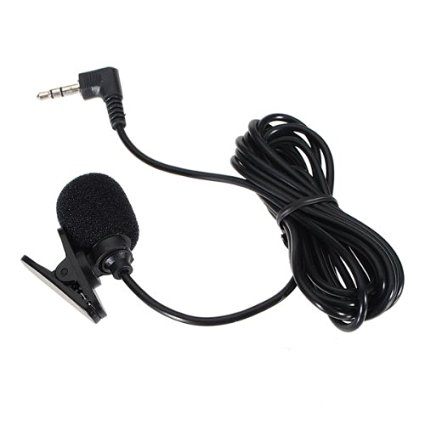
\includegraphics[scale=0.30]{../images/hardware/mic.jpg}
    \caption{Micrófono}
    \label{fig:microfono}
  \end{center}
\end{figure}

\bigskip

\begin{itemize}
 \item \textbf{Tarjeta SD (4GB)}
 \begin{itemize}
  \item Descripción: Tarjeta SD que permite la carga del SO en la Raspberry Pi.
  \item Especificaciónes: \url{https://www.amazon.com/SanDisk-Class-Memory-SDSDB-004G-B35-Change/dp/B000WQKOQM}
  \item Precio: ~12 Euros
 \end{itemize}
\end{itemize}
\begin{figure}[!ht]
  \begin{center}
    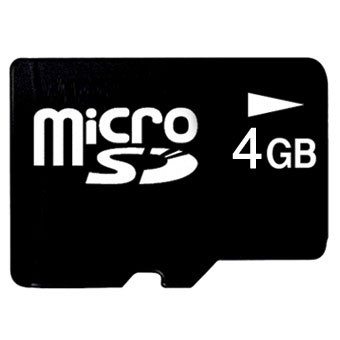
\includegraphics[scale=0.10]{../images/hardware/sd.jpg}
    \caption{Tarjeta SD}
    \label{fig:tarjetasd}
  \end{center}
\end{figure}


\begin{itemize}
 \item \textbf{Memoria USB (16GB)}
 \begin{itemize}
  \item Descripción: Memoria que contiene el SO de la Raspberry Pi.
  \item Especificaciónes: \url{http://tiendas.mediamarkt.es/p/pendrive-de-16gb-sandisk-cruzer-blade-usb-2.0-ultracompacto-en-color-negro-y-rojo-1117065}
  \item Precio: 5 Euros
 \end{itemize}
\end{itemize}
\begin{figure}[!ht]
  \begin{center}
    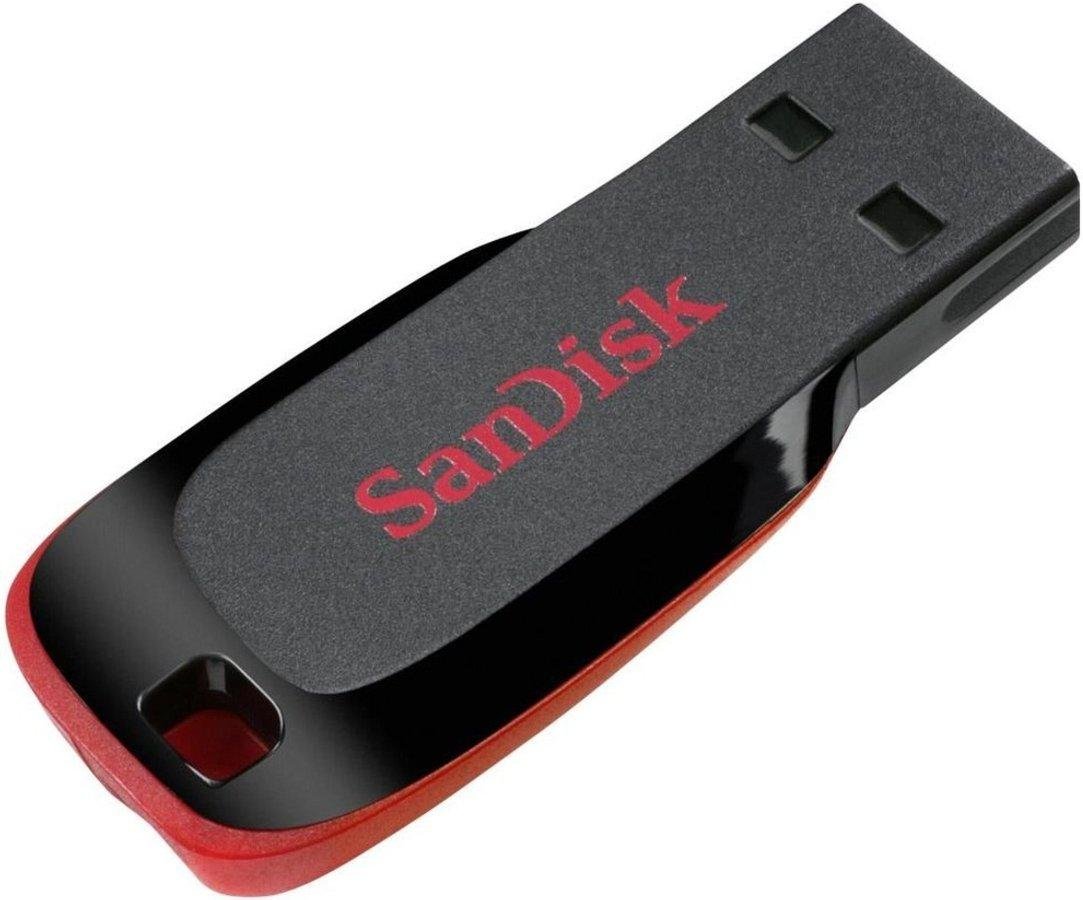
\includegraphics[scale=0.05]{../images/hardware/usbdrive.jpg}
    \caption{Memoria USB}
    \label{fig:soundcard}
  \end{center}
\end{figure}

\begin{itemize}
 \item \textbf{VPS Amazon EC2}
 \begin{itemize}
  \item Descripción: Conjunto de servidores que conforman el proyecto, de tipo \textbf{t2.micro}
  \begin{itemize}
    \item 1 instancia para la plataforma IOT.
    \item 1 instancia para la base de datos de almacenamiento masivo.
    \item 1 instancia para el visualizador de datos.
    \item 1 instancia para el servidor web.
  \end{itemize}
  \item Especificaciónes: \url{https://aws.amazon.com/es/ec2/instance-types/}
  \item Precio: Este tipo de servidores son gratuitos en amazon EC2 durante un año, por lo que no existe coste a priori.
 \end{itemize}
\end{itemize}

Por tanto, por un total de unos 65 Euros aproximadamente podemos disponer de todo lo necesario para construir el proyecto.
